\chapter{Musical intonation: building on Auto-Tune and millenia of music history}
\label{chap:intonation}
This chapter provides an overview of the concept of musical intonation. It provides a musical background for the design of the automatic pitch correction system proposed in this thesis. It starts with definitions of intonation and related terms such as frequency, pitch, and interval. It then introduces two standard conceptualizations of musical intonation. The first defines precise mathematical formulas involving ratios, while the second is based on empirical observations, involving complex interactions between physics of sound, psychoacoustics, and musical culture. This chapter discusses how relative merits of these two conceptualizations have been debated for millenia, and relates them to musical practices in cultures ranging from European Classical music and Indian Raga to Blues and 21$^{st}$ century pop music. It finds that the way a musical culture thinks about musical intonation has a large impact on the way musicians create music. This chapter then introduces Antares Auto-Tune, one of the music industry standards for pitch correction, and the first of its kind. It relates the underlying assumptions about singing in tune that informed its design to the way it is used by musicians, both amateur and professional. Auto-Tune falls strictly into the ratio-based camp of the debate. This turns out very suitable some musical styles, even creating opportunities for new ways of making music, but is not suitable for others. This chapter discusses the various ways in which Auto-Tune is used---some of which have been surprising---along with its reception, ranging from positive to negative. The chapter concludes by considering how incorporating the empirical perspective on singing in tune would lead to a different design, and how this could improve the musicality of automatic pitch correction. 

\section{What is musical intonation?} 
Defining musical intonation requires that we first define \textit{frequency}, \textit{period}, and \textit{pitch}. Hass describes these concepts in the context of acoustics. ``Some sound waves are periodic, in that the change from equilibrium (average atmospheric pressure) to maximum compression to maximum rarefaction back to equilibrium is repetitive. The 'round trip' back to the starting point just described is called a cycle.'' The common measurement unit for frequency is in cycles per second or simply cps. One hertz (abbr. Hz, named after the 19th C. physicist) [...] equals 1 cycle per second. ``They are synonymous and interchangeable values used to convey frequency.'' \cite[][Ch.~1, Sec.~4--5]{hass2019introduction} Periodic sound waves are the focus of this thesis, as they are the ones where a listener will hear a pitch, as in singing voice, instead of a noise as in consonants in speech or ocean waves. 

Parncutt \textit{et al.} define pitch by comparing it to frequency: 
\begin{quotation}In general, [pitch] is not the same as [frequency]. We use the term \textit{pitch} in the psycho-acoustic sense of the experience of how high or low a tone sounds. It is a purely subjective parameter---an experience of the listener that can depend on several different physical parameters.'' \cite[][p.~477]{parncutt2018psychocultural}\end{quotation}

The Cambridge Online Dictionaries (6/12/2020) define musical intonation as the degree to which the notes of a piece of music are played or sung exactly in  tune,  e.g.,  ``The  violinist  had  good  intonation,  and a wonderful pure tone.'' It defines \textit{in tune} as: singing or playing notes that are at the right pitch (= level) or that agree with others being sung or played. 

The Dictionaries definition implies that musical intonation can be experienced only when two or more tones are played together, either simultaneously or in succession. The relationship between two tones is referred to as an \textit{interval}.

Unlike the definition above, which focuses on the listeners' perspective, Parncutt \textit{et al.} define intonation by musicians' actions: ``the real-time adjustment of (fundamental) frequencies in music performance.'' \cite[p.~477]{parncutt2018psychocultural} They elaborate this definition as it relates to limits of auditory perception, inharmonicity of musical tones, pitch as a subjective value versus frequency as an objective metric, and complexity and subjectivity in music.

Precisely and comprehensively defining musical intonation is challenging. First, the subjective component makes it difficult to directly measure intonation without feedback from listeners. Second, the relationship between frequency and pitch is complex, as described in section \ref{sec:empirical}. Third, a performer dynamically adjusts intonation over time. In some musical contexts such as jazz improvisation, a musician can transform locally bad intonation into globally good intonation. Bassist Victor Wooten famously teaches this to students. He uses an exercise where a student who plays a note that sounds out of key slides it over a half step in either direction, which then sounds good. ``You’re never more than a half step away from a right note,'' he says. ``It keeps [the students] from being afraid of being wrong. And if they are wrong, it’s only the note, not everything else. The music doesn’t have to stop.'' \cite{Freddy2020}

\section{Measuring musical intonation}
\label{sec:ratio}
Despite the challenges in precisely defining musical intonation, the concept has been the subject of research and debate for millenia. Developing a way of measuring intervals, or the relationship between tones, is key to studying intonation. This section introduces two contrasting conceptualizations: ratio-based and empirically derived. This section focuses on Western music because the author's training is in this culture, but it also mentions intonation systems from other cultures. One of the themes of this thesis is that the proposed system can be personalized to any musical cultures.

\begin{figure*}[t!]
$\begin{array}{rl}
    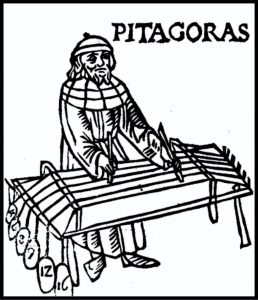
\includegraphics[height=1.9in]{images/en_harmonik_pitagoras.jpg} &
    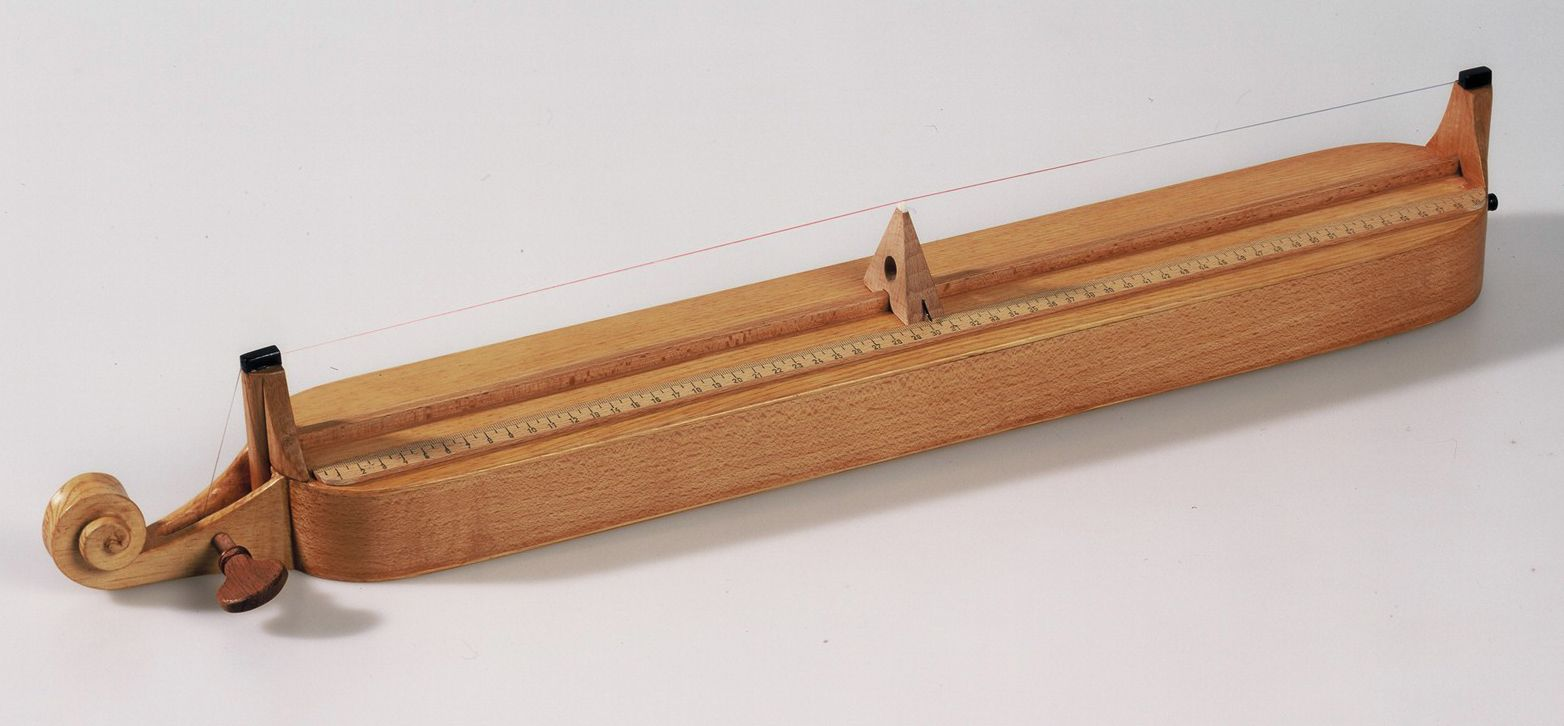
\includegraphics[height=1.9in]{images/monochord.jpg}\\
    \multicolumn{2}{c}{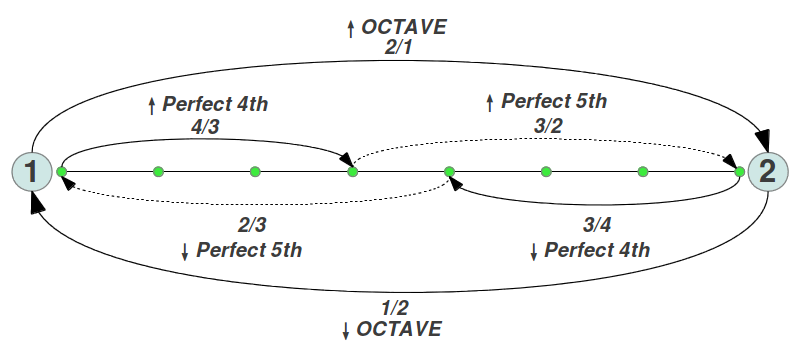
\includegraphics[height=2.3in]{images/sacred_geometry_octave_fourth_fifth.png}}
\end{array}$
\caption[]{\label{fig:pythagoras}Illustrations of Pythagoras' technique using a monochord to generate musical intervals. Pressing down a string at specific distances produces substrings with lengths whose ratios to the full string length are 2:1 for an octave, 3:2 for a fifth, etc... The intervals can be heard by plucking the string. The mathematician is depicted in (a). The image was found in a book by Middle Ages music theorist Franchino Gaffurio (1492--1480?) \cite{pitagoras}. (b) is a modern-day replica of the monochord instrument \cite{monochord}. (c) shows the exact locations where the string should be pressed to produce an octave, a perfect fifth, and a perfect fourth.}
\end{figure*}

\subsection{Ratio-based measures of intonation}
\label{sec:ratio}
One natural approach to measuring an interval is to calculate the ratio between the two fundamental frequencies. Fundamental frequency is the lowest frequency of the waveform. Use of \textit{fundamental} frequency is an important distinction in natural waveforms, which are usually periodic at many different values. Fundamental frequency often roughly corresponds to the pitch the listener perceives, as the next section describes in more detail.

Pythagorean and just intonation are closely related ratio-based systems that define intervals as in tune, or \textit{pure}, when the length of their shared periodicity is minimal. An octave has a ratio of 2:1, and a fifth a ratio of 3:2, making these two intervals the most pure after the unison, which has a ratio of 1:1. Pythagorean intonation is attributed by legend to the mathematician Pythagoras (sixth century B.C.), along with the invention of the monochord, a one-stringed instrument used by Pythagoreans and acoustical scientists up through the Middle Ages \cite[][Ch.~2, p.~2 and Ch.~4, p.~42]{weiss2007music}. Figure \ref{fig:pythagoras} shows depictions of Pythagoras using a monochord, a modern-day replica of a monochord, and a chart showing how to produce pure musical intervals. 

In Pythagorean intonation, every interval is constructed from octaves and fifths, and is formulated as $2**a3**b:1$, where $a$ and $b$ are whole numbers. This leads to the concern of large ratios when using intervals beyond the fifth and the fourth. For example, a major third is $81/64:1$. Just intonation addresses these concerns by adding powers of $5$. This enables a smaller ratio for the major third, namely, $4/5$ \cite{parncutt2018psychocultural}.

Just intonation was used in Europe during the Renaissance, as shown in writings by composer and music theorist Gioseffo Zarlino's \textit{Istitutioni harmoniche} (1558). Zarlino was an advocate of using as many pure intervals as possible \cite{goldman1991new}. In fact, when music is complex enough that there are multiple intervals occurring at the same time---for example, in polyphonic music---it is often mathematically impossible to make all intervals pure. Keeping intervals pure becomes even more difficult on fixed-pitch instruments such as keyboards, where it is not possible to adjust a tone's frequency based on the interval that is being played. Zarlino defended Just intonation against another tuning system---equal temperament---that was advocated for by other theorists such as Franchino Gafurius (1451-1524) and Faber Stapulensis (1455-1537). Equal temperament involved replacing pure intervals with equally spaced ones, though the ratio between them is irrational, approaching $2^\frac{n}{12}$, where $n$ is a whole number \cite{goldman1991new}. They represented a practical compromise that often sounded quite good. The equal-tempered scale became more established in the late 18th century \cite{equaltemperament}.

In contemporary Western music, Pythagorean, Just, and Equal-tempered scales remain prominent. The Equal-tempered scale is commonly used for tuning fixed-pitch instruments, but Pythagorean and Just systems are commonly taught to musicians who play of continuous-pitched instruments such as violin or voice. New understanding of the physics of sound provides incentive to use pure intervals. Pitched waveforms are represented as sine tones at the fundamental frequencies. Intervals are represented as their sums. Small-integer ratios minimize \textit{roughness} and \textit{beats}: periodic oscillations in amplitude caused by constructive and destructive interference of the signals, which are considered undesirable.

\subsection{Empirically derived measures of intonation}
\label{sec:empirical}
An alternative to the ratio-based conceptualization of musical intonation, as old as its counterpart, is the empirical approach. Parncutt \textit{et al.} refer to Aristoxenus' three books entitled ``Elements of Harmony'', where he \begin{quotation}argued on the basis of musical experience and intuition that the basic elements of musical structure---intervals, scales, tuning, melody---do not depend on arithmetic proportions, as the Pythagoreans claimed, but on what we today would call auditory psychology: processes of auditory perception, cognition, memory, and recall. To understand music, we have to perceive it. To understand the musical effect or function of an interval, we have to listen to it, not make abstract calculations. To understand how melodies work, we have to perceive, remember, and reproduce them. Musicians are not aware of ratios as they perform melodies. Interval sizes vary on a continuous scale and do not generally correspond to mathematically idealized ratios \cite[][p.~475]{parncutt2018psychocultural}.\end{quotation} 

Parncutt \textit{et al.} argue in favor of the empirical approach. This section lists some of the arguments, but I encourage the reader to refer to the article for a comprehensive list and more details. 

First, studies measuring interval sizes in Western tonal musical performances on continous-pitch instruments such as voice or violin find much variety in musical interval sizes both above and below the ratio based and equal-tempered intervals. For example, Devaney \textit{et al.} find such deviations in polyphonic choral music performed by professional-level musicians \cite{devaney2011intonation}. More generally, studies tend to report normal, unimodal distributions around the twelve equal divisions of the octave. The octave that is divided into twelve is slightly larger than 2:1. The theoretical Just and Pythagorean variants are found to lie well within the distributions. The studies also show that performers tend to stretch larger intervals, compress smaller intervals, and play sharper if they are soloists. Researchers hypothesize that performers might exaggerate intonation patters for stylistic purposes. 

Second, physical, fundamental frequency and perceived pitch differ most of the time. One reason for this is nonlinearity in the cochlea’s spectrum analysis. However, perceived pitch also changes based on intensity, register, timbre, and masking effects when multiple sounds are played simultaneously. Perceived pitch can differ from frequency as much as two semitones.

Third, rich timbres, inharmonicity---the fact that the overtone frequencies are often not exact integer ratios of the fundamental frequency---and randomization of phase via overlapping of the direct sound and its reflections, make most beats and roughness inaudible in practice.

Fourth, there are physical limits to how precisely the human auditory system can detect pitch, for example, if a note is short. Physical limits also apply to how precise a performer can be.

Fifth, a performer's pitch can drift over time, either on purpose or through random variation. This means that the ratio between frequencies is changing over time, not locked into a specific value.

Parncutt \textit{et al.} conclude that \begin{quotation}[m]usical intervals are not ratios, nor are they magical mathematical entities. They are learned, approximate, perceptual distances. They emerge from a multi-generational perceptual-historical process, mediated by the physical properties of musical tones and the physiological and psychological properties and limitations of the human auditory system.\end{quotation}
 
\subsection{Outcomes in music}
The conceptualizations of musical intonation described above played an significant role in forming musical language and conventions. This section provides a few examples of how musicians' conceptualization of intonation led them to compose and perform music in a certain way. It is by no means comprehensive, but serves as background for considering how the design of music technology might affect what kind of music users are able to make with it or will choose to make. 

\subsubsection{Ancient Greek philosophy as a basis for Western tonality}
The first example is how the Ancient Greek concept of pure intervals along with abstraction of musical events led to simple structures that formed the basis for Classical Western tonality. Burkholder \textit{et al.} describe how ``[f]or Pythagoras and his followers, numbers were the key to the universe, and music was inseparable from numbers.’’ Pure intervals were linked to \textit{harmonia}, the unification of parts in an orderly whole. \begin{quotation}Through this flexible concept---which could encompass mathematical proportions, philosophical ideas, or the structure of society as well as a particular musical interval, scale type, or style of melody---Greek writers perceived music as a reflection of the order of the universe. \cite[][Ch.~1, p.~13]{burkholder2010history}\end{quotation}

Burkholder \textit{et al.} show that the history of music in medieval Europe is built on these concepts. Music in medieval Europe was intertwined with the history of the Christian Church, which was influential across the continent. The church drew on Greek philosophy in music theory, adopting the concept of perfect intervals relating to God \cite[Ch.~2, p.~22]{burkholder2010history}. In Gregorian chant, a \textit{parallel organum} consists of a principal voice chanting the main melody, and of an \textit{organal voice} that moves in exact parallel motion a fifth below. The Fifth was considered consonant, perfect, and beautiful, and superior to other intervals. The very simple structure of parallel fifths, however, led singers to innovate by experimenting with other intervals and breaking from perfect parallel motion. For example, when singers innovated by using parallel motion at a fourth instead of at a fifth, they introduced delays in one of the voices to avoid tritone intervals, which were considered extremely dissonant. This move away from exact parallel motion opened the door to polyphony, which grew more complex over time and formed the basis of Western tonal harmony \cite[Ch.~5, p.~86]{burkholder2010history}.

Burkholder \textit{et al.} also describe how Aristoxenus, in his \textit{Harmonic Elements}, \begin{quotation}distinguishes between \textit{continuous} movement of the voice, gliding up and down in speech, and \textit{diastematic} [...] movement, in which the voice moved between sustained pitches separated by a discrete intervals. A melody consists of a series of notes, each on a single pitch; an interval is formed between two notes of different pitch; and a scale is a series of three or more different pitches in ascending or descending order. Such seemingly simple definitions established a firm basis for Greek music and all leader music theory. \cite[][Ch.~1, p.~15]{burkholder2010history}\end{quotation}

Both the restriction of musical intervals according to Pythagoras' conceptualization of intervals as ratios and the abstraction of pitch variations into notes according to Aristoxenus were simple conceptualizations of complex musical events. This simplification led to the ability to build complex harmonic structures and polyphony such as one finds in Beethoven's symphonies from a discrete set of musical ``building blocks''. The equal-tempered scale was a further simplification of the ``building blocks'', sacrificing small pitch nuances to enable increasingly complex harmonic modulations. 

\subsubsection{Classical Indian theory}
Classical Western Tonality can be contrasted to musical cultures that prioritize nuances in pitch and rhythm over harmonic modulations, choosing to use a more complex set of ``building blocks''. Classical Indian theory is one such example. 

Ramanna writes about \textit{Ragas}, or scales: ``In principle, an octave can be divided into any number of parts, but musical value of a raga restricts these to a maximum of only seven out of altogether 22 intervals. […] The frequency ratios of the \textit{Swaras} (notes) play the most important part in the creation of a raga or a scale. ’’ \cite[][p.~897]{ramanna1995structure} Classical Indian music theory varies by region. Ramanna writes about the Venkatamakhin scheme, where ``the […] octave is divided into 7 Swaras of different intervals in 72 different ways. The 72 combinations [form] the basic Ragas from which other Ragas can be recognized. Though some appear identical, they differ in the way they are played.’’ \cite[][p.~898]{ramanna1995structure} Furthermore, ``The change of tonic in a piece of Karnatic music is strictly forbidden. This has, as, perhaps, come about due to the fact that any change of tonic requires a retuning of all the notes in a non-even temperament system.’’ \cite[p.~899]{ramanna1995structure}

Arnold, writing from a Western perspective, proposes that \begin{quotation}La théorie musicale ancienne de l'Inde, exposée integralement dans les premiers traités sanscrits sur la musique, et qui s'intéresse à la notion de consonance, aux échelles musicales et à leurs arrangements systématiques préservant les différences enharmoniques entre les positions tonales des notes, constitue la formulation la plus incisive du système d'intonation juste qui ait jamais été proposée. [Ancient Indian music theory, integrally formulated in the first Sanscrit treatises on music, and that focuses on concepts of consonance, musical scales and their systematic arrangements preserving enharmonic differences between the notes’ tonal positions, constitutes the most incisive formulation of the Just intonation that has ever been proposed.] \cite[translated from French][p.~11]{arnold1985intonation}.\end{quotation}

Classical Indian music theory also has a divine component. Chatterji writes about the Northern Indian \textit{Raga-Ragini} theory:\begin{quotation}[T]he entire \textit{Raga} world derived from six ragas and thirty-six raginis. These original six ragas are considered to be of divine origin. They each have six `wives’ or feminine ragas-(aginis) and these in turn have `putras’ or sons. \parencite[][p.~362]{chatterji1958indian}\end{quotation}

\subsubsection{Blues}
Blues is a musical genre developed by African Americans in the early 20th century. Blues became by the 1960s one of the most important influences on popular music in the United States \cite{blues}. Palmer writes that ``[t]he African music from which the blues ultimately derived came to what is now the Southern United States with the first African slaves. These Africans had belonged to a number of different tribal and linguistic groups, Each of which had its own musical traditions.’’ \cite[][p.~25]{palmer1981deep} Some traditions had for many centuries had contact with Berber and Arab cultures in the North of the desert. The vocal music in these areas reflected the Middle East’s tendency for long, tortuous melodic lines and formal solo singing. In other cultures, music tended to consist of group singing in call and response form with multiple overlapping melodies and percussion orchestras playing dazzlingly complex polyrhythms. Harmony was also used: ``Not the periodic resolving Harmony of European music but the parallel Melodies song of third, fourth, or fifth away from each other.’’ \cite[][p.~27]{palmer1981deep} Alper describes how slaves were not allowed to sing music from their homelands, but incorporated performance practices into the musical forms that they were permitted to perform. \cite{alper2005flexibility}. Ultimately, what developed was a set of template chord progressions that were repeated during a piece. Twelve-bar blues is a widely used template \cite{alper2005flexibility}. These chord progressions use periodic resolving harmony of European music. However, the chord progression is not the main focus of the music, but rather provides a predictable structure on which instrumentalists and singers can improvise complex melodies or rhythms, or add personal nuances such as vocal intonation. These aspects of Blues relate closely to the African style. One nuance Blues is notorious for is intentional off-key singing \cite{autotuneBritannica}, which is an example of a musical practice that does not fit into the Just or Pythagorean conceptualization of intonation, but rather in the empirical, cultural conceptualization described by Aristoxenus.

\subsubsection{21$^{st}$ century Pop music}
Peres analyzes pop songs released between 2011 and early 2016 using the concept of \textit{sonic syntax}. He defines sonic syntax as ``a musical grammar that relies on manipulation of timbre, sonic
density (the presence and amplitude of frequencies across the sonic spectrum at any given
moment), and rhythmic intensity.'' \cite[][p.~2]{peres2016sonic} Sections and subsections of a song function as sonic setup, buildup, or peak. Electronic dance music was the first popular genre to use sonic syntax as the driving structural feature. Recent pop music has adopted a similar same syntax, with the consequence of tonality becoming a secondary component in musical structure. Peres describes how this musical innovation in pop based on developments in audio techonology. ``Modern technology allows record producers nearly-unlimited control over timbre, which they have used to create new forms of musical expression.'' \cite[][p.~36]{peres2016sonic} The ability to control timbre and small nuances leaves room for the development of musical subcultures and expressive nuances. Section \ref{sec:autotune} describes how Auto-Tune is commonly used in contemporary music as an effect, and can be considered a subculture. Given the close relationship between intonation and timbre, the question arises of how a differently designed system might be used by musicians.

\subsection{Conceptualization of intonation in this thesis}
Ratio-based conceptualization of musical intervals has shown much merit in development and understanding of sophisticated musical structures. However, it does not prioritize subtle but significant nuances found in many musical genres. 

This thesis conceptualizes intonation based on the empirical approach described in \ref{sec:empirical}. It limits its scope to intonation of singing voice in relation to a backing track, or recorded accompaniment. It defines intonation as adjustment of (fundamental) frequencies in music performance so that the pitches in the voice ``agree'' with the content in the backing track. It defines this agreement not via the proximity of the intervals to ratios of fundamental frequencies belonging to a discrete, pre-defined set, but based on proximity to patterns found in the given musical tradition. This definition is built on the assumption that musical traditions have developed based on physical properties of sound and psychoacoustics, providing either purity or roughness in intervals, which provide a stimulating and expressive sound to the listeners. 

\section{Antares Auto-Tune}
\label{sec:autotune}
This section summarizes the functionality of Auto-Tune so that we can understand how it models musical intonation. It starts with a brief history of Auto-Tune for context. 

\subsection{A brief history}
For two decades, Antares Auto-Tune has been the world standard for professional pitch correction. The way that other available tools (e.g.,  Melodyne) model pitch closely resembles that of Auto-Tune.

Andy Hildebrand founded Jupiter Systems, which later became Antares Audio Technology, in 1997. He got his PhD in electrical engineering at the University of Illinois, with a focus on signal processing. His full-time job involved signal processing on seismic data for oil exploration. In an interview in 2016 with Eckard \cite{eckard2016}, he wrote: 
\begin{quotation}Around 1995 I was at a trade show, it was me and a couple partners, and we were with a person who was distributing our products. His wife was there, and we were talking about what products would be interesting to do next. His wife said, ``Well, Andy, why don't you make me a box that would have me sing in tune?'' I looked around at the table, and everyone just stared at their lunch plates, they didn't say a word.

So I thought, ``boy, that's a lousy idea.'' About eight or nine months into the year, I'd gone to work for a different project, and I came back to that idea, I said, ``you know, that's pretty straightforward to do, I'll do that.'' At the same trade show a year later I had producers ripping it out of my hands.
\end{quotation}
In the interview, Hildebrand described Western music as having a long history of innovations, and placed Auto-Tune into that timeline. He expressed surprise at the fact that artists often did not use the Auto-Tune software as intended, to discretely fix a singer's pitch, but instead used extreme settings that produce a robotic effect.

\subsection{How does Auto-Tune work?}
The Auto-Tune Pro Manual \cite{antares:2018} describes the program's functionality in detail. This section focuses on the features that are relevant to the thesis. Auto-Tune features two modes of operation---\textit{Auto Mode}, which is optimized for automatic (optionally, real-time) adjustments, and \textit{Graph Mode}, which provides a user interface for precise, manual editing of the pitch and timing. Auto Mode is most relevant as it is designed to be used in a similar context to the proposed program. Graph Mode enables the user to be as musically refined and nuanced as they wish to be, but is not automatic and requires more extensive use of an interface.   

Auto-Tune in Auto Mode takes as input a well-isolated, monophonic sound source. It continuously adjusts the input pitch towards a target pitch. The target pitch is the closest scale tone as determined by the current scale settings. The default scale is the chromatic, equal-tempered scale, but the user can customize the set of notes that is used by specifying the key and the scale. These can also be automatically detected using MIDI. Furthermore, the user can customize the (fixed) frequency of every note.

One of the most important parameters in Auto-Tune is the \textit{Retune Speed}, which controls how rapidly the pitch correction is applied to the incoming audio. The units are milliseconds. If set to zero, the pitch is immediately shifted to the target pitch, completely suppressing any vibrato or deviations in pitch. A setting between 10 and 50 milliseconds is commonly used for producing a more natural-sounding effect. There is always a tradeoff between remaining close to the scale and preserving pitch variation. Some additional functionalities help address unwanted artifacts. One is the \textit{Humanize} function, which adjusts Retune Speed based on the length of the note. The Retune Speed is reduced on longer notes to prevent a static pitch, but kept fast for the short notes so that the melodic contour is accurate. Another is \textit{Flex-Tune}. This control helps note transitions be less abrupt by only applying pitch correction when the performer approaches the target note. Controls also exist to amplify existing vibrato or to add a synthesized one. Finally, controls exist to preserve the singer's formant---their spectral shaping that results from the acoustic resonance of their vocal tract---or even change it to sound like they have a longer or shorter throat. Voices are put into five categories: Soprano, Alto/Tenor, Bass, Instrument, Bass Instrument. This categorization also helps preserve a natural formant. 

\section{Auto-Tune's ratio-based conceptualization of musical interval}
\label{sec:interval-conceptualization-design}
Auto-Tune's model of pitch originates directly from the ratio conceptualization of intervals introduced in Section \ref{sec:ratio}. We can conjecture a set of assumptions that underlie the way the program applies corrections. The first assumption is that perceived pitch and fundamental frequency can be treated as equivalent. This assumption is evident from the fact that Auto-Tune is described as a pitch-correction program instead of a fundamental-frequency-correction program \cite{antares:2018}, meaning that the corrections apply at the perceptual level. A second assumption is that a note's proximity to a small set of frequencies---by default, the twelve notes in the equal-tempered scale---is considered accurate and, by extension, in tune. A third assumption is that masking and interference from the backing track does not provide essential information for the pitch corrections: Auto-Tune only processes the vocal track without referring to the backing track. A fourth assumption is that the center pitch in every note is remains constant throughout, except during note transitions at the beginning and end. Pitch bending is not explicitly modeled. 

\subsection{Modeling tradeoffs and negative reception}
While the simple model behind Auto-Tune makes it possible to design a program that consistently produces reliable results, it is worth pondering what nuances are lost in the process.\footnote{Parncutt \textit{et al.} recommended that ``Computer scientists [...] resist the temptation to develop and implement models of musical structure based on frequency ratios.'' I personally spent much of my early PhD thinking about how such a model could be developed, but found the task difficult. I synthesized four-part harmony with intervals based on just or Pythagorean intonation and only produced dissonant results.} First, while the concept of intervals as ratios is useful, shifting frequencies so that the ratios of their fundamental frequencies exactly correspond to the small number of acceptable values removes both desired and erroneous pitch variations without discrimination. One can argue that, in the process, part of the social phenomenon that is music is lost: the part of music that consists of a shared auditory culture, where artists and listeners learn to appreciate specific pitch patterns in specific contexts, and become part of a musical community. Second, results of psychoacoustics are ignored in favor of theoretical models of musical intonation that do not correspond to what proficient musicians have been shown to do in practice. Third, the richness of vocal timbre and of interaction between the vocals and backing track is ignored. 

Fourth, many musical practices and even cultures are left out. Early reception of the Auto-Tune program showed concern for this reason. As described in \textit{Encyclopaedia Britannica}, 
\begin{quotation}Critics noted that Auto-Tune had disrupted a long and important history of intentional off-key singing, a technique that was particularly prevalent in the blues, a style that became the backbone of much of popular music in the present day. Blues singers traditionally played with pitch to express feelings such as longing or yearning, to punch up a nastier lyric, or to make the lyrics sound more suggestive. For example, Mick Jagger’s vocals on \textit{Sweet Virginia,} from the seminal Rolling Stones album \textit{Exile on Main Street}, were sung almost totally flat for the purpose of achieving a certain effect.'' \cite{autotuneBritannica}
\end{quotation} 
There is also no modeling of Aristoxenus' diastematic pitch movement, of tortuous melodies as found in Arab-influenced music, or of off-tune singing in blues.

\subsubsection{A visual analogy}
I personally find that it is easy to get lost while discussing aesthetics in the context of music, so I provide a crude analogy. Human height approximately follows a multimodal normal distribution. Suppose somebody determines that a good height for a human corresponds to one of these modes, and develops technology to make all people have one of these heights. The result would be that many people would appear relatively natural when encountered individually, but would produce an uncanny effect when encountered as a group: People would have exactly the same height. 

\subsubsection{Negative contemporary opinions}
Among amateur singers, Auto-Tune used in the fully automatic mode on apps such as Smule produces a robotic effect not always popular among users. One Smule user writes about a plug-in that includes Auto-Tune: ``please whatever you do don’t use Popstar/Super Pop on a song that is not meant for [Auto-Tune]. Nothing kills the mood faster LOL.'' \cite{smule-blog} This comment indicates that the effect is so strong that users omit using it unless a song sounds good with the obviously audible effect. 

Though this thesis focuses on automatic pitch correction for amateur musicians, it is interesting to consider how professional artists adopted Auto-Tune. As described in more detail in Section \ref{sec:professional}, Auto-Tune has become a popular effect among professional singers. One can contrast Miley Cyrus's Auto-Tuned voice in \textit{Party in the USA} at 0:09 and 0:43 to her natural voice \textit{The Backyard Sessions - ``Jolene''}\footnote{\url{https://youtu.be/wOwblaKmyVw}, accessed 06/20/2020}. It is not uncommon to hear criticism regarding ``excessive use of Auto-Tune'', e.g., \cite{katz2014}, making singing voice sound overly processed. 

\subsection{Adoption by professional artists and positive reception}
\label{sec:professional}
The initial goal of Auto-Tune was to automatically help people sing more in tune. \textit{Sunday Morning} Maroon 5 or \textit{Toxic} by Britney Spears both used Auto-tune in the expected manner. A listener might not notice the effect unless they are aware of it and put some thought into it.

Others turned the settings to extreme values to develop new musical styles. An early example is \textit{Buy U a Drank (Shawty Snappin')} by T-Pain (feat. Yung Joc), starting at 0:02. Recent examples in R\&B include \textit{Die For You} by The Weeknd, contrasting heavy Auto-Tune at 1:24 with a rich voice at 0:28, and \textit{Work} by Rihanna and Drake, at 0:09 and 1:00, where the latter example makes her voice sound like a theremin. In rap, one example is \textit{What The Price} by Migos. It uses different settings in overlapping voices, at 0:17, 0:26, and 0:44. In electropop, \textit{Anything could happen} by Ellie Goulding uses different settings at 0:00, 0:08, and 2:28. To hear a song with Auto-Tune versus without, Ke\$ha's \textit{Die Young} can be heard as the original production or \textit{deconstructed}, with her natural voice. In Electronic Dance Music, Daft Punk \textit{Harder, better, faster, stronger} uses Auto-Tune at 1:37. 

\section{How millenia of music theory and the design of Auto-Tune inform this thesis}
Auto-Tune is an early system for automatic pitch correction. Its invention and commercialization has led to widespread usage, development of new musical effects used in multiple genres, and positive and negative reactions. Auto-Tune created new musical opportunities, but also left out important musical practices and nuances from many traditions. The analysis of the assumptions behind the design of Auto-Tune and how they affected the way the program works and is used by musicians provides a useful background for this thesis. The system proposed in this thesis is designed based on the empirical conceptualization of musical intonation. It strives to incorporate and even encourage use of subtle pitch nuances. Chapter \ref{chap:tech-background} describes the process of designing a computer program for automatic pitch correction.

While this chapter has provided ample reason to consider an empirical approach to automatic pitch correction, or to develop a more complex model of intonation, one question arises. Does moving towards an empirical representation of musical intonation force us to discard an elegant mathematical and physical theory? Parncutt \textit{et al.} argue that this is not the case. 
\begin{quotation}Physics is often thought of as an `exact science' because it is dominated by mathematical theory. But mathematics is also an excellent tool for dealing with inexactness. Music theory is often considered mathematical and therefore exact. In fact, the quantities considered in applied mathematics vary along a spectrum from very exact to very approximate. The number ratios that correspond to musical intervals also lie somewhere along that spectrum.''
\end{quotation}

%\subsection{What do we want? My research question} A program that automatically adjusts pitch of singing voice given a fixed backing track. It should sound more in tune after the adjustment without sacrificing the overall quality of the sound. This leaves many open questions. What is in tune? What aspects of overall quality do we wish to preserve? What is automatic?

%Use patterns from performances. What is the best way for the program to access audio features and context to make good predictions? How do we evaluate? How should we represent pitch: notes, frames? How do we apply the shifts? How do we preserve natural sound? What is our scope? Hobby karaoke, post-processing.

% This is a figure in landscape orientation
%\begin{sidewaysfigure}
%\includegraphics[width=\textwidth]{figures/exampleFigure.png}
%\caption{This is another example Figure, rotated to landscape orientation.}
%\label{LandscapeFigure}
%\end{sidewaysfigure}
